\qcor targets an execution model whereby application execution is directed by the host with access to an attached quantum device. Applications consist of purely classical and quantum-classical expressions and routines. Figure \ref{fig:exec_model} illustrates \qcor's execution model. Applications are compiled and execute both host and quantum device code. The host device executes \qcor library calls which may consist of both classical and quantum tasks. When the host encounters a quantum kernel within the quantum-classical task, the kernel is passed to the quantum device controller. \qcor quantum-classical tasks are executed asynchronously, meaning, the host initiates the task and continues to the next statement or expression in the application without waiting for the quantum-classical task to complete.
% Execution on the host is asynchronous to execution on the quantum device. 
\qcor exposes initialization, synchronization, execution, and memory management library application programming interfaces (api's) to the user that enable a wide variety of hybrid quantum-classical use cases.

\begin{figure*}
 \centering
 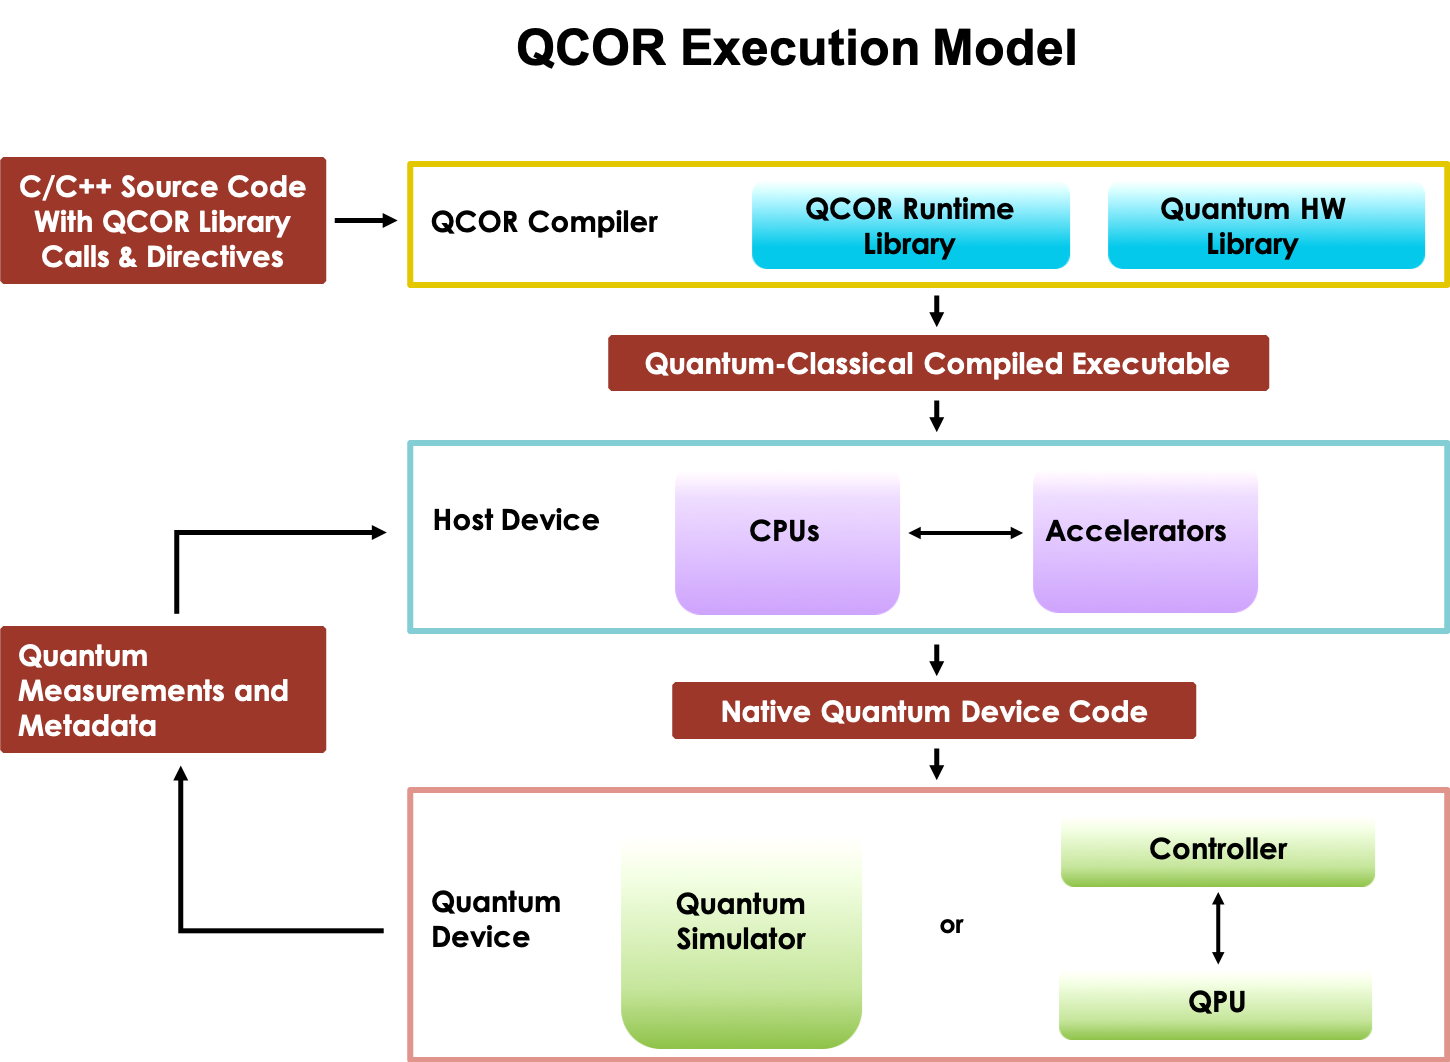
\includegraphics[width=5in,height=4in]{figures/Execution_Model_Illustration_v3.png}
  \caption{Diagram of \qcor Execution Model}
  \label{fig:exec_model}
\end{figure*}


\subsection{\textbf{Quantum Kernels}}\label{subsec:kernel}
\qcor extends \CorCpp by allowing the programmer to define functions, called \FUNC{kernels}, that, when called, are executed asynchronously on the quantum device. A \FUNC{kernel} is defined using the \_\_qpu\_\_ declaration specifier. A \FUNC{kernel} can optionally accept native or user defined \CorCpp datatypes as arguments, as well as datatypes within the \qcor language extension.

The \FUNC{kernel} function body should be a sequence of instructions on qbits and can also include control flow statements and predefined macros.  This circuit level expressiveness can be implemented using languages like \textit{QASM}, \textit{XASM}, and \textit{Quill}. 
%TODO: Insert footnotes or citations for qasm, xasm and quill

%The sample code below illustrates \FUNC{kernel} usage in a \CorCpp program.
%TODO: insert example
